%\documentclass[11pt]{proc}
\documentclass[preprint,10pt]{sigplanconf}

\usepackage{amsmath}
\usepackage{url}
\usepackage{graphicx}

\begin{document}

\title{Emscripten: An LLVM-to-JavaScript Compiler}
\conferenceinfo{Splash '11}{??-2011, Portland.} 
\copyrightyear{2011} 
\copyrightdata{[to be supplied]} 
\titlebanner{}        % These are ignored unless
\preprintfooter{}   % 'preprint' option specified.
\authorinfo{Alon Zakai}
           {Mozilla}
           {azakai@mozilla.com}

\maketitle

%\title{Emscripten: An LLVM-to-JavaScript Compiler}
%\subtitle{}
%\authorinfo{Alon Zakai}
%           {Mozilla}
%           {azakai@mozilla.com}
%\author{Alon Zakai \\ Mozilla \\ \url{azakai@mozilla.com}}
%\maketitle

\begin{abstract}
We present Emscripten, a compiler from LLVM (Low Level Virtual Machine) assembly to JavaScript. This
opens up two avenues for running code written
in languages other than JavaScript on the web: (1) Compile code directly into LLVM assembly, and
then compile that into JavaScript using Emscripten, or (2) Compile
a language's entire runtime into LLVM and then JavaScript, as in the previous
approach, and then use the compiled runtime to run code written in that language. For example, the
former approach can work for C and C++, while the latter can work for Python; all three
examples open up new opportunities for running code on the web.

Emscripten itself is written in JavaScript and is available under the MIT
license (a permissive open source license), at \url{http://www.emscripten.org}.
As a compiler from LLVM to JavaScript, the challenges in designing
Emscripten are somewhat the reverse of the norm -- one must go from a low-level
assembly into a high-level language, and recreate parts of the original
high-level structure of the code that were lost in the compilation to
low-level LLVM. We detail the methods used in
Emscripten to deal with those challenges, and in particular present and prove
the validity of Emscripten's Relooper
algorithm, which recreates high-level loop structures from low-level
branching data.
\end{abstract}

%\category{CR-number}{subcategory}{third-level}

%\terms
%term1, term2

%\keywords
%keyword1, keyword2

\bigskip

%\copyright 2011 Alon Zakai. License: Creative Commons Attribution-ShareAlike (CC BY-SA), \url{http://creativecommons.org/licenses/by-sa/3.0/}

\section{Introduction}

Since the mid 1990's, JavaScript~\cite{js} has been present in most web browsers (sometimes
with minor variations and under slightly different names, e.g., JScript in Internet
Explorer), and today it is
well-supported on essentially all web browsers, from desktop browsers like
Internet Explorer, Firefox, Chrome and Safari, to mobile browsers on smartphones
and tablets. Together with HTML and CSS, JavaScript forms the standards-based
foundation of the web.

Running other programming languages on the web has been suggested many times,
and browser plugins have allowed doing so, e.g., via the Java
and Flash plugins. However, plugins must be manually installed and do not integrate in
a perfect way with the outside HTML. Perhaps more problematic is that they cannot run
at all on some platforms, for example, Java and Flash cannot run on iOS devices such as the iPhone
and iPad. For those reasons, JavaScript remains
the primary programming language of the web.

There are, however, reasonable motivations for running code from
other programming languages on the web, for example, if one has a large
amount of existing code already written in another language, or if one
simply has a strong preference for another language and perhaps is
more productive in it. As a consequence, there has been work on tools to compile languages
\textbf{into} JavaScript. Since JavaScript is present in essentially all web
browsers, by compiling one's language of choice into JavaScript, one
can still generate content that will run practically everywhere.

Examples of the approach of compiling into JavaScript include
the Google Web Toolkit~\cite{gwt}, which compiles Java into JavaScript;
Pyjamas\footnote{\url{http://pyjs.org/}}, which compiles Python into JavaScript;
SCM2JS \cite{hop}, which compiles Scheme to JavaScript,
Links \cite{links}, which compiles an ML-like language into JavaScript;
and AFAX \cite{afax}, which compiles F\# to JavaScript;
see also \cite{ashkenas} for additional examples.
While useful, such tools usually only allow a subset of the original language to
be compiled. For example, multithreaded code (with shared memory) is
not possible on the web, so compiling code of that sort is
not directly possible. There are also often limitations of the conversion
process, for example, Pyjamas compiles Python to JavaScript in a nearly
1-to-1 manner, and as a consequence the underlying semantics are those of JavaScript,
not Python, so for example division of integers can yield unexpected results
(it should yield an integer in Python 2.x,
but in JavaScript and in Pyjamas a floating-point number can be generated).

In this paper we present another project along those lines: \textbf{Emscripten},
which compiles LLVM (Low Level Virtual Machine\footnote{\url{http://llvm.org/}}) assembly into JavaScript.
LLVM is a compiler project primarily focused on C, C++ and
Objective-C. It compiles those languages through a \emph{frontend} (the
main ones of which are Clang and LLVM-GCC) into the
LLVM intermediary representation (which can be machine-readable
bitcode, or human-readable assembly), and then passes it
through a \emph{backend} which generates actual machine code for a particular
architecture. Emscripten plays the role of a backend which targets JavaScript.

By using Emscripten, potentially many languages can be
run on the web, using one of the following methods:
\begin{itemize}
\item Compile \textbf{code} in a language recognized by one of the existing LLVM frontends
      into LLVM, and then compile that
      into JavaScript using Emscripten. Frontends for various languages
      exist, including many of the most popular programming languages such as C and
      C++, and also various new and emerging languages (e.g., Rust\footnote{\url{https://github.com/graydon/rust/}}).
\item Compile the \textbf{runtime} used to parse and execute code in
      a particular language into LLVM, then compile that into JavaScript using
      Emscripten. It is then possible to run code in that runtime on the web.
      This is a useful approach if
      a language's runtime is written in a language for which an LLVM
      frontend exists, but the language itself has no such frontend. For
      example, there is currently no frontend for Python, however
      it is possible to compile CPython -- the standard implementation of
      Python, written in C -- into JavaScript, and run Python code on that
      (see Section~\ref{sec:examples}).
\end{itemize}

From a technical standpoint, one challenge in designing and implementing
Emscripten is that it compiles a low-level language -- LLVM assembly -- into
a high-level one -- JavaScript. This is somewhat the reverse of the usual
situation one is in when building a compiler, and leads to some unique
difficulties. For example, to get good performance in JavaScript one must
use natural JavaScript code flow structures, like loops and ifs, but
those structures do not exist in LLVM assembly (instead, what is present
there is a `soup of code fragments': blocks of code with branching information
but no high-level structure).
Emscripten must therefore reconstruct a high-level
representation from the low-level data it receives.

In theory that issue could have been avoided by compiling a higher-level
language into JavaScript. For example, if compiling Java into JavaScript
(as the Google Web Toolkit does), then one can benefit from the fact
that Java's loops, ifs and so forth generally have a very direct parallel
in JavaScript. But of course the downside in that approach is it yields a
compiler only for Java. In Section~\ref{sec:relooper}
we present the `Relooper' algorithm, which generates high-level loop structures from the low-level
branching data present in LLVM assembly. It is similar to loop recovery algorithms used in decompilation
(see, for example, \cite{Cifuentes98assemblyto}, \cite{pro97}).
The main difference between the Relooper and standard loop recovery algorithms
is that the Relooper generates loops in a different language than that which was compiled originally, whereas
decompilers generally assume they are returning to the original language. The Relooper's
goal is not to accurately recreate the original source code, but rather to generate
native JavaScript control flow structures, which can then be implemented
efficiently in modern JavaScript engines.

Another challenge in Emscripten is to maintain accuracy (that is, to
keep the results of the compiled code the same as the original)
while not sacrificing performance. LLVM assembly
is an abstraction of how modern CPUs are programmed for, and its basic
operations are not all directly possible in JavaScript. For example, if in
LLVM we are to add two unsigned 8-bit numbers $x$ and $y$, with overflowing (e.g., 255
plus 1 should give 0), then there is no single operation in JavaScript which
can do this -- we cannot just write $x+y$, as that would use the normal JavaScript
semantics. It is possible to emulate a CPU in JavaScript, however doing so
is very slow. Emscripten's approach is to allow such emulation, but to try to
use it as little as possible, and to provide tools that help one find out
which parts of the compiled code actually need such full emulation.

We conclude this introduction with a list of this paper's main contributions:
\begin{itemize}
\item We describe Emscripten itself, during
      which we detail its approach in compiling LLVM into JavaScript.
\item We give details of Emscripten's Relooper algorithm, mentioned earlier, which generates
      high-level loop structures from low-level branching data, and prove
      its validity.
\end{itemize}
In addition, the following are the main contributions of Emscripten
itself, that to our knowledge were not previously possible:
\begin{itemize}
\item It allows compiling a very large subset of C and C++ code into
      JavaScript, which can then be run on the web.
\item By compiling their runtimes, it allows running languages such as Python
      on the web (with their normal semantics).
\end{itemize}

The remainder of this paper is structured as follows. In Section~\ref{sec:compapp} we
describe the approach Emscripten takes to compiling LLVM assembly into JavaScript,
and show some benchmark data.
In Section~\ref{sec:emarch} we describe Emscripten's internal design and in
particular elaborate on the Relooper algorithm.
In Section~\ref{sec:examples} we give several example uses of
Emscripten. In Section~\ref{sec:summary} we summarize and give directions for future
work.

\section{Compilation Approach}
\label{sec:compapp}

Let us begin by considering what the challenge is, when we want to compile LLVM assembly
into JavaScript. Assume we are given the
following simple example of a C program:
\begin{verbatim}
  #include <stdio.h>
  int main()
  {
    int sum = 0;
    for (int i = 1; i <= 100; i++)
      sum += i;
    printf("1+...+100=%d\n", sum);
    return 0;
  }
\end{verbatim}
This program calculates the sum of the integers from 1 to 100. When
compiled by Clang, the generated LLVM
assembly code includes the following:
\label{code:examplellvm}
\begin{verbatim}
@.str = private constant [14 x i8]
        c"1+...+100=%d\0A\00"

define i32 @main() {
  %1 = alloca i32, align 4
  %sum = alloca i32, align 4
  %i = alloca i32, align 4
  store i32 0, i32* %1
  store i32 0, i32* %sum, align 4
  store i32 1, i32* %i, align 4
  br label %2

; <label>:2
  %3 = load i32* %i, align 4
  %4 = icmp sle i32 %3, 100
  br i1 %4, label %5, label %12

; <label>:5
  %6 = load i32* %i, align 4
  %7 = load i32* %sum, align 4
  %8 = add nsw i32 %7, %6
  store i32 %8, i32* %sum, align 4
  br label %9

; <label>:9
  %10 = load i32* %i, align 4
  %11 = add nsw i32 %10, 1
  store i32 %11, i32* %i, align 4
  br label %2

; <label>:12
  %13 = load i32* %sum, align 4
  %14 = call i32 (i8*, ...)*
        @printf(i8* getelementptr inbounds
          ([14 x i8]* @.str, i32 0, i32 0),
          i32 %13)
  ret i32 0
}
\end{verbatim}
At first glance, this may look more difficult to translate into
JavaScript than the original C++. However, compiling C++ in
general would require writing code to handle preprocessing,
classes, templates, and all the idiosyncrasies and complexities
of C++. LLVM assembly, while more verbose in this example, is
lower-level and simpler to work on. Compiling it also has the benefit we
mentioned earlier, which
is one of the main goals of Emscripten, that it allows many languages can
be compiled into LLVM and not just C++.

A detailed overview of LLVM assembly is beyond our scope here (see \url{http://llvm.org/docs/LangRef.html}). Briefly,
though, the example assembly above can be seen to define a
function main(), then allocate some values on the stack (alloca),
then load and store various values (load and store). We do not have
the high-level code structure as we had in C++ (with a loop), instead
we have labeled code fragments, called LLVM basic blocks, and code flow moves
from one to another by branch (br) instructions. (Label 2 is the
condition check in the loop; label 5 is the body, label 9 is the
increment, and label 12 is the final part of the function, outside
of the loop).
Conditional branches
can depend on calculations, for example the results of comparing
two values (icmp). Other numerical operations include addition (add).
Finally, printf is called (call). The challenge, then, is to convert
this and things like it into JavaScript.

In general, Emscripten's main approach is to translate each line of LLVM
assembly into JavaScript, 1 to 1, into `normal' JavaScript
as much as possible. So, for example, an \emph{add} operation becomes
a normal JavaScript addition, a function call becomes a JavaScript
function call, etc. This 1 to 1 translation generates JavaScript
that resembles the original assembly code, for example, the LLVM assembly code shown
before for main() would be compiled into the following:
\label{code:example}
\begin{verbatim}
function _main() {
  var __stackBase__  = STACKTOP;
  STACKTOP += 12;
  var __label__ = -1;
  while(1) switch(__label__) {
    case -1:
      var $1 = __stackBase__;
      var $sum = __stackBase__+4;
      var $i = __stackBase__+8;
      HEAP[$1] = 0;
      HEAP[$sum] = 0;
      HEAP[$i] = 0;
      __label__ = 0; break;
    case 0:
      var $3 = HEAP[$i];
      var $4 = $3 <= 100;
      if ($4) { __label__ = 1; break; }
      else    { __label__ = 2; break; }
    case 1:
      var $6 = HEAP[$i];
      var $7 = HEAP[$sum];
      var $8 = $7 + $6;
      HEAP[$sum] = $8;
      __label__ = 3; break;
    case 3:
      var $10 = HEAP[$i];
      var $11 = $10 + 1;
      HEAP[$i] = $11;
      __label__ = 0; break;
    case 2:
      var $13 = HEAP[$sum];
      var $14 = _printf(__str, $13);
      STACKTOP = __stackBase__;
      return 0;
  }
}
\end{verbatim}
Some things
to take notice of:
\begin{itemize}
\item A switch-in-a-loop construction is used in order to let the flow
      of execution move between basic blocks of code in an arbitrary manner: We set
      \emph{\_\_label\_\_} to the (numerical representation of the) label of
      the basic block we want to reach, and do a break, which leads to the proper
      basic block being reached. Inside each basic block, every line of code corresponds to a line of
      LLVM assembly, generally in a very straightforward manner. 
\item Memory is implemented by \emph{HEAP}, a JavaScript array. Reading from
      memory is a read from that array, and writing to memory is a write.
      \emph{STACKTOP} is the current position of the stack. (Note that we
      allocate 4 memory locations for 32-bit integers on the stack, but only 
      write to 1 of them. See Section~\ref{sec:lsc} for why.)
\item LLVM assembly functions become JavaScript functions, and function calls
      are normal JavaScript function calls. In general, we attempt to generate
      as `normal' JavaScript as possible.
\item We implemented the LLVM \emph{add} operation using simple addition in JavaScript.
      As mentioned earlier, the semantics of that code are not entirely identical to
      those of the original LLVM assembly code (in this case, overflows will have very
      different effects). We will explain Emscripten's approach to that problem in
      Section~\ref{sssec:realworldcode}.
\end{itemize}

\subsection{Performance}
\label{sec:perf}

In this section we will deal with several topics regarding
Emscripten's approach to generating high-performance JavaScript code.

\subsubsection{Load-Store Consistency (LSC)}
\label{sec:lsc}

We saw before that Emscripten's memory usage allocates the usual number
of bytes on the stack for variables (4 bytes for a 32-bit integer, etc.).
However, we only wrote values into the first location, which appeared odd.
We will now see the reason for that.

To get there, we must first step back, and note that
Emscripten does not aim to achieve perfect compatibility with all possible
LLVM assembly (and correspondingly, with all possible C or C++ code, etc.);
instead, Emscripten targets a large subset of LLVM assembly code, which is portable
and does not make crucial assumptions about the underlying CPU architecture
on which the code is meant to run. That subset is meant to encompass the
vast majority of real-world code that would be compiled into LLVM,
while also being compilable into very
performant JavaScript.

More specifically, Emscripten assumes that the LLVM assembly code it is
compiling has \textbf{Load-Store Consistency} (LSC), which is the requirement that
after a value with a specific type is written to a memory location, loads from
that memory location will be of the same type (until a value with a different
type is written there).
Normal C and C++
code generally does so: If $x$ is a variable containing a 32-bit floating
point number, then both loads and stores of $x$ will be of 32-bit floating
point values, and not 16-bit unsigned integers or anything else.

To see why this is important for performance, consider the following
C code fragment, which does \emph{not} have LSC:
\begin{verbatim}
  int x = 12345;
  printf("first byte: %d\n", *((char*)&x));
\end{verbatim}
Assuming an architecture with more than 8 bits, this code will read
the first byte of \emph{x}. (This might, for example, be used to detect the
endianness of the CPU.) To compile this into JavaScript in
a way that will run properly, we must do more than a single operation
for either the read or the write, for example we could do this:
\begin{verbatim}
  var x_value = 12345;
  var x_addr = stackAlloc(4);
  HEAP[x_addr]   = (x_value >> 0) & 255;
  HEAP[x_addr+1] = (x_value >> 8) & 255;
  HEAP[x_addr+2] = (x_value >> 16) & 255;
  HEAP[x_addr+3] = (x_value >> 24) & 255;
  [...]
  printf("first byte: %d\n", HEAP[x_addr]);
\end{verbatim}
Here we allocate space for the value of \emph{x} on the stack, and
store that address in \emph{x\_addr}. The stack itself is part of
the `memory space', which is the array \emph{HEAP}. In order for
the read on the final line to give the proper value, we must go to
the effort of doing 4 store operations, each of the value of a
particular byte. In other words, \emph{HEAP} is an array of bytes,
and for each store into memory, we must deconstruct the value into
bytes.\footnote{Note that we can use JavaScript typed arrays with a shared memory
buffer, which would work as expected, assuming (1) we are running
in a JavaScript engine which supports typed arrays, and (2) we
are running on a CPU with the same architecture as we expect. This
is therefore dangerous as the generated code may run differently on
different JavaScript engines and different CPUs.
Emscripten currently has optional experimental support for typed arrays.}

Alternatively, we can store the value in a single operation, and
deconstruct into bytes as we load. This will be faster in some
cases and slower in others, but is still more overhead
than we would like, generally speaking -- for if the code \textbf{does} have
LSC, then we can translate that code fragment into
the far more optimal
\begin{verbatim}
  var x_value = 12345;
  var x_addr = stackAlloc(4);
  HEAP[x_addr] = x_value;
  [...]
  printf("first byte: %d\n", HEAP[x_addr]);
\end{verbatim}
(Note that even this can be optimized even more -- we can store
\emph{x} in a normal JavaScript variable. We will discuss such
optimizations in Section \ref{sec:codeopt}; for now we are
just clarifying why it is useful to assume we are compiling code
that has LSC.)

In practice the vast majority of C and C++ code does have LSC. Exceptions
do exist, however, for example:
\begin{itemize}
\item Code that detects CPU features like endianness, the behavior of floats, etc. In general such code can be disabled
      before running it through Emscripten, as it is not actually needed.
\item \emph{memset} and related functions typically work on values of one kind,
      regardless of the underlying values. For example, memset may write 64-bit
      values on a 64-bit CPU since that is usually faster than writing individual
      bytes. This tends to
      not be a problem, as with \emph{memset} the most common case is setting to
      0, and with \emph{memcpy}, the values end up copied properly anyhow (with
      a proper implementation of \emph{memcpy} in Emscripten's generated code).
\item Even LSC-obeying C or C++ code may turn into LLVM assembly that does not,
      after being optimized. For example, when storing two 32-bit integers constants into
      adjoining locations in a structure, the optimizer may generate a single
      64-bit store of an appropriate constant. In other words, optimization can
      generate nonportable code, which runs faster on the current CPU, but
      nowhere else. Emscripten currently assumes that optimizations of this form
      are not being used.
\end{itemize}
In practice it may be hard to know if code has LSC or not, and requiring
a time-consuming code audit is obviously impractical. Emscripten therefore has
a compilation option, SAFE\_HEAP, which generates code that checks that LSC holds, and warns if it
doesn't. It also warns about other memory-related issues like
reading from memory before a value was written (somewhat similarly to tools
like Valgrind\footnote{\url{http://valgrind.org/}}). When such problems are detected, possible solutions are to ignore the issue (if it has no actual
consequences), or alter the source code.

Note that it is somewhat wasteful to allocate 4 memory locations for
a 32-bit integer, and use only one of them. It is possible to change
that behavior with the QUANTUM\_SIZE parameter to Emscripten, however,
the difficulty is that LLVM assembly has hardcoded values that depend on
the usual memory sizes being used. We are looking into modifications
to LLVM itself to remedy that.

\subsubsection{Emulating Code Semantics}
\label{sssec:realworldcode}

As mentioned in the introduction, the semantics of LLVM assembly and JavaScript are not identical: The former
is very close to that of a modern CPU, while the latter is a high-level
dynamic language. Both are of course Turing-complete, so it is possible to
precisely emulate each in the other, but doing so with good performance is
more challenging. For example, if we want to convert
\begin{verbatim}
  add i8 %1, %2
\end{verbatim}
(add two 8-bit integers) to JavaScript, then to be completely accurate we must emulate the
exact same behavior, in particular, we must handle overflows properly, which would not be the case if we just implement
this as $\%1 + \%2$ in JavaScript. For example, with inputs of $255$ and $1$, the
correct output is 0, but simple addition in JavaScript will give us 256. We
can of course emulate the proper behavior by adding additional code.
This however significantly degrades performance,
because modern JavaScript engines can often translate something like $z = x + y$ into
native code containing a single instruction (or very close to that), but if instead we had
something like $z = (x + y)\&255$ (in order to correct overflows), the JavaScript engine
would need to generate additional code to perform the AND operation.\footnote{
In theory, the JavaScript engine could determine that we are implicitly working
on 8-bit values here, and generate machine code that no longer needs the AND operation.
However, most or all modern JavaScript engines have just two internal numeric types, doubles and
32-bit integers. This is so because they are tuned for `normal' JavaScript code
on the web, which in most cases is served well by just those two types.

In addition, even if JavaScript engines did analyze code containing $\&255$, etc.,
in order to deduce that a variable can be implemented
as an 8-bit integer, there is a cost to including all the necessary $\&255$ text
in the script, because code size is a significant factor on the web. Adding even
a few characters for every single mathematic operation, in a large JavaScript file,
could add up to a significant increase in download size.}

Emscripten's approach to this problem is to allow the generation of both accurate code,
that is identical in behavior to LLVM assembly, and inaccurate code which is
faster. In practice, most addition operations in LLVM do not overflow,
and can simply be translated into $\%1 + \%2$. Emscripten
provides tools that make it straightforward to find which code does require
the slower, more accurate code, and to generate that code in those locations, as follows:
\begin{itemize}
\item Compile the code using Emscripten with special options that generate runtime checking.
      CHECK\_OVERFLOWS adds runtime checks for integer overflows, CHECK\_SIGNS
      checks for signing issues (the behavior of signed and unsigned integers can
      be different, and JavaScript does not natively support that difference), and
      CHECK\_ROUNDINGS checks for rounding issues (in C and C++, the convention is
      to round towards 0, while in JavaScript there is no simple operation that does
      the same).
\item Run the compiled code on a representative sample of inputs, and notice which
      lines are warned about by the runtime checks.
\item Recompile the code, telling Emscripten to add corrections (using CORRECT\_SIGNS, CORRECT\_OVERFLOWS
      or CORRECT\_ROUNDINGS) only on the specific lines that actually need it.
\end{itemize}

This method is not guaranteed to work, as if we do not run on a truly representative
sample of possible inputs, we may not compile with all necessary corrections. It is
of course possible to compile with all corrections applied to all the code, to make
sure things will work properly (this is the default compilation setting), however, in
practice the procedure above works quite well, and results in code is significantly faster.

\subsubsection{Emscripten Code Optimizations}
\label{sec:codeopt}

When comparing the example program from page~\pageref{code:example},
the generated code was fairly complicated
and cumbersome, and unsurprisingly it performs quite poorly. There
are two main reasons for that: First, that the code is simply
unoptimized -- there are many variables declared when fewer could
suffice, for example, and second, that the code does not use `normal'
JavaScript, which JavaScript engines are optimized for -- it
stores all variables in an array (not normal JavaScript variables),
and it controls the flow of execution using a switch-in-a-loop, not
normal JavaScript loops and ifs.

Emscripten's approach to generating fast-performing code is as
follows. Emscripten doesn't do any
optimizations that can be done by other tools:
LLVM can be used to perform optimizations before Emscripten, and
the Closure Compiler\footnote{\url{http://code.google.com/closure/compiler/}}
can perform optimizations on the generated JavaScript afterwards. Those
tools will perform standard useful optimizations like removing unneeded variables, dead code elimination,
function inlining, etc.
That leaves two major optimizations that are left for Emscripten
to perform:
\begin{itemize}
\item \textbf{Variable nativization}: Convert variables
      that are on the stack -- which is implemented using addresses in the \emph{HEAP} array
      as mentioned earlier -- into native JavaScript variables (that is to say, \emph{var x;} and so forth). In general,
      a variable will be nativized unless it is used
      outside that function, e.g., if its address is taken and stored somewhere
      or passed to another function. When optimizing, Emscripten tries to nativize
      as many variables as possible.
\item \textbf{Relooping}: Recreate high-level loop and if structures
      from the low-level code block data that appears in LLVM assembly.
      We describe Emscripten's Relooper algorithm in Section~\ref{sec:relooper}.
\end{itemize}

When run with Emscripten's optimizations, the code on page \pageref{code:example} looks
like this:
\begin{verbatim}
function _main() {
  var __label__;
  var $1;
  var $sum;
  var $i;
  $1 = 0;
  $sum = 0;
  $i = 0;
  $2$2: while(1) {
    var $3 = $i;
    var $4 = $3 <= 100;
    if (!($4)) { __label__ = 2; break $2$2; }
    var $6 = $i;
    var $7 = $sum;
    var $8 = $7 + $6;
    $sum = $8;
    var $10 = $i;
    var $11 = $10 + 1;
    $i = $11;
    __label__ = 0; continue $2$2;
  }
  var $13 = $sum;
  var $14 = _printf(__str, $13);
  return 0;
}
\end{verbatim}
If in addition the Closure Compiler is run on that output, we get
\begin{verbatim}
function K() {
  var a, b;
  b = a = 0;
  a:for(;;) {
    if(!(b <= 100)) {
      break a
    }
    a += b;
    b += 1;
  }
  _printf(J, a);
  return 0;
}
\end{verbatim}
which is fairly close to the original C++ (the differences, of
having the loop's condition inside the loop instead of inside
the for() expression at the top of the original loop, are not important to performance). Thus, it is possible
to recreate the original high-level structure of the code that
was compiled into LLVM assembly.

\subsection{Benchmarks}
\label{sec:benchmarks}

We will now take a look at some performance benchmarks:

\bigskip

\begin{tabular}{ l | c | c | c || c }
  \hline
  \textbf{benchmark} & \textbf{SM}    & \textbf{V8}    & \textbf{gcc} & \textbf{ratio} \\
  \hline
  fannkuch (10)      & 1.158          & \textbf{0.931} & 0.231       &  4.04 \\
  fasta (2100000)    & \textbf{1.115} & 1.128          & 0.452       &  2.47 \\
  primes             & \textbf{1.443} & 3.194          & 0.438       &  3.29 \\
  raytrace (7,256)   & \textbf{1.930} & 2.944          & 0.228       &  8.46 \\
  dlmalloc (400,400) & 5.050          & \textbf{1.880} & 0.315       &  5.97 \\
  \hline
\end{tabular}

\bigskip

The first column is the name of the benchmark, and in parentheses any
parameters used in running it. The source code to all the benchmarks
can be found at \url{https://github.com/kripken/emscripten/tree/master/tests}
(each in a separate file with its name, except for `primes', which is
embedded inside runner.py in the function test\_primes). A brief summary of
the benchmarks is as follows:
\begin{itemize}
\item \textbf{fannkuch} and \textbf{fasta} are commonly-known benchmarks, appearing for example
      on the Computer Language Benchmarks Game\footnote{\url{http://shootout.alioth.debian.org/}}.
      They use a mix of mathematic operations (integer in the former, floating-point in the latter) and memory access.
\item \textbf{primes} is the simplest benchmark in terms of code. It is basically just a tiny loop that calculates prime numbers.
\item \textbf{raytrace} is real-world code, from the sphereflake raytracer\footnote{\url{http://ompf.org/ray/sphereflake/}}. This benchmark has a combination of memory access and floating-point math.
\item \textbf{dlmalloc} (Doug Lea's malloc\footnote{\url{http://en.wikipedia.org/wiki/Malloc#dlmalloc_and_its_derivatives}}) is a well-known real-world implementation of malloc and free. This benchmark does a large amount of calls to malloc and free in an intermixed way, which tests memory access and integer calculations. 
\end{itemize}

Returning to the table of results, the second
column is the elapsed time (in seconds) when running the compiled code (generated using all Emscripten and LLVM
optimizations as well as the Closure Compiler) in the SpiderMonkey JavaScript
engine (specifically the JaegerMonkey branch, checked out June 15th, 2011).
The third column is the elapsed time when running the same JavaScript code in the V8 JavaScript engine
(checked out Jun 15th, 2011). In both the second and third column lower values
are better; the best of the two is in bold.
The fourth column is the elapsed time when running the original code compiled with \emph{gcc -O3},
using GCC 4.4.4. The last column is the ratio, that is, how much slower the JavaScript code
(running in the faster of the two engines for that test) is
when compared to gcc. All the tests were run on a MacBook Pro with
an Intel i7 CPU clocked at 2.66GHz, running on Ubuntu 10.04.

Clearly the results greatly vary by the benchmark, with the generated JavaScript running from 2.47 to 8.46 times
slower. There are also significant differences between the two JavaScript engines, with each better
at some of the benchmarks.
It appears that code that does simple numerical operations -- like
the primes test -- can run fairly fast, while code that has a lot of memory
accesses, for example due to using structures -- like the raytrace test --
will be slower. (The main issue with structures is that Emscripten does not
`nativize' them yet, as it does to simple local variables.)

Being 2.47 to 8.46 times slower than the most-optimized C++ code
is a significant slowdown, but it is still more than fast enough for
many purposes, and the main point of course is that the code can run
anywhere the web can be accessed. Further work on Emscripten is expected to
improve the speed as well, as are improvements to LLVM, the Closure
Compiler, and JavaScript engines themselves; see further discussion
in the Summary.

\subsection{Limitations}

Emscripten's compilation approach, as has been described in this Section so far,
is to generate `natural' JavaScript, as close as possible to normal JavaScript
on the web, so that modern JavaScript engines perform well on it. In particular,
we try to generate `normal' JavaScript operations, like regular addition and
multiplication and so forth. This is a very
different approach than, say, emulating a CPU on a low level, or for the case
of LLVM, writing an LLVM bitcode interpreter in JavaScript. The latter approach
has the benefit of being able to run virtually any compiled code, at the cost
of speed, whereas Emscripten makes a tradeoff in the other direction. We will
now give a summary of some of the limitations of Emscripten's approach.

\begin{itemize}
\item \textbf{64-bit Integers}: JavaScript numbers are all 64-bit doubles, with engines
      typically implementing them as 32-bit integers where possible for speed.
      A consequence of this is that it is impossible to directly implement
      64-bit integers in JavaScript, as integer values larger than 32 bits will become doubles,
      with only 53 bits for the significand. Thus, when Emscripten uses normal
      JavaScript addition and so forth for 64-bit integers, it runs the risk of
      rounding effects. This could be solved by emulating 64-bit integers,
      but it would be much slower than native code.
\item \textbf{Multithreading}: JavaScript has Web Workers, which are additional
      threads (or processes) that communicate via message passing. There is no
      shared state in this model, which means that it is not directly possible
      to compile multithreaded code in C++ into JavaScript. A partial solution
      could be to emulate threads, without Workers, by manually controlling
      which blocks of code run (a variation on the switch in a loop construction
      mentioned earlier) and manually switching between threads every so often.
      However, in that case there would not be any utilization
      of additional CPU cores, and furthermore performance would be slow due to not
      using normal JavaScript loops.
\end{itemize}

After seeing these limitations, it is worth noting that some advanced LLVM instructions turn out to be
surprisingly easy to implement. For example, C++ exceptions are represented in
LLVM by \emph{invoke} and \emph{unwind}, where \emph{invoke} is a call to a function that will
potentially trigger an \emph{unwind}, and \emph{unwind} returns to the earliest invoke.
If one were to implement those
in a typical compiler, doing so would require careful work. In Emscripten, however,
it is possible to do so using JavaScript exceptions in a straightforward manner:
\emph{invoke} becomes a function call wrapped in a \emph{try} block, and \emph{unwind}
becomes \emph{throw}. This is a case where compiling to a high-level language turns
out to be quite convenient.

\section{Emscripten's Architecture}
\label{sec:emarch}

In the previous section we saw a general overview of Emscripten's approach
to compiling LLVM assembly code into JavaScript. We will now get into more detail
into how Emscripten itself is implemented.

Emscripten is written in JavaScript. The primary reason for that decision
was convenience: Two simple examples of the benefits of that approach are that (1)
the compiler can create JavaScript objects that represent constant structures from the original
assembly code, and convert them to a string using JSON.stringify()
in a trivial manner,
and (2) the compiler can simplify numerical operations by simply
eval()ing the code (so ``1+2'' would become ``3'', etc.). In both examples,
the development of Emscripten was made simpler by having the exact same environment
during compilation as the executing code will have. This also helps in more
complex ways, for example when the same code needs to be run at compile time
and at runtime, and makes various dynamic compilation techniques possible in the future.

Emscripten's compilation has three main phases:
\begin{itemize}
\item The \textbf{intertyper}, which converts from LLVM assembly into
      Emscripten's internal representation.
\item The \textbf{analyzer}, which inspects the internal representation
      and generates various useful information for the final phase,
      including type and variable information, stack usage analysis,
      optional data for optimizations
      (variable nativization and relooping), etc.
\item The \textbf{jsifier}, which does the final conversion of the
      internal representation plus additional analyzed data into JavaScript.
\end{itemize}

\subsection{The Runtime Environment}
\label{sec:runtime}

Code generated from Emscripten is meant to run in a JavaScript engine,
typically in a web browser. This has implications for the kind of
runtime environment we can generate for it, for example, there is no
direct access to the local filesystem.

Emscripten comes with a partial implementation of a C library,
mostly written from scratch in JavaScript, with parts compiled from an
existing C library\footnote{newlib, \url{http://sourceware.org/newlib/}}. Some aspects of the runtime environment, as
implemented in that C library, are:
\begin{itemize}
\item An emulated filesystem is available, with files stored in memory.
\item Emscripten allows writing pixel data to an HTML5 canvas element,
      using a subset of the SDL API. That is, one can write an application in C or C++ using
      SDL, and that same application can be compiled normally and run
      locally, or compiled using Emscripten and run on the web. See, for
      example, Emscripten's raytracing demo at \url{http://syntensity.com/static/raytrace.html}.
\item \emph{sbrk()} is implemented using the \emph{HEAP} array which
      was mentioned previously. This allows a normal \emph{malloc()}
      implementation written in C to be compiled to JavaScript.
\end{itemize}

\subsection{The Relooper: Recreating high-level loop structures}
\label{sec:relooper}

The Relooper the most complex module in Emscripten. It receives
a `soup of blocks', which is a set of labeled fragments of code, each
ending with a branch operation, and the goal is to generate normal
high-level JavaScript code flow structures such as loops and ifs.
Generating such code structures is essential to producing good-performing code,
since JavaScript engines are tuned to run such code very quickly (for
example, a tracing JIT as in SpiderMonkey will only trace normal loops).

Returning to the LLVM assembly code on page~\pageref{code:examplellvm}, it
has the following structure (where arrows denote potential paths of execution):

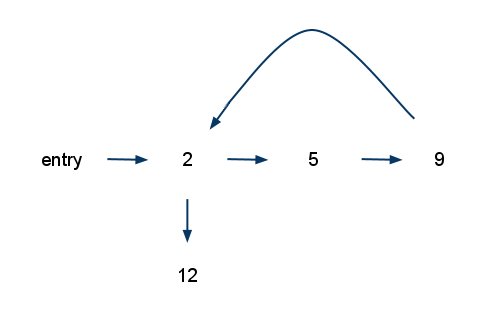
\includegraphics[width=80mm]{graph.png}

In this simple example, it is fairly straightforward to see that a natural way to implement it
using normal loop structures is
\newpage
\begin{verbatim}
ENTRY
while (true) do
  2
  if (condition) break
  5
  9
12
\end{verbatim}
In general though, this is not always easy or even practical -- there may
not be a straightforward high-level loop structure corresponding to the low-level one, if
for example the original C code relied heavily on \emph{goto} instructions.
In practice, however, almost all real-world C and C++ code tends to
be amenable to loop recreation.

We now begin to describe the Relooper algorithm. As mentioned before, it takes as input a `soup of labeled LLVM blocks' as described above,
and generates a structured set of Emscripten code blocks, which are each a set of LLVM blocks
with some logical structure. For simplicity we call LLVM blocks `labels' and Emscripten
blocks `blocks' in the following.

There are three types of Emscripten blocks:
\begin{itemize}
\item \textbf{Simple block}: A block with
  \begin{itemize}
  \item One \textbf{Internal} label, and
  \item a \textbf{Next}
      block, which the internal label branches to. The block is later
      translated simply into the code for that label, and the Next
      block appears right after it.
  \end{itemize}
\item \textbf{Loop}: A block that represents a basic loop, comprised of
      two internal sub-blocks:
  \begin{itemize}
  \item \textbf{Inner}: A block that will appear inside
        the loop, i.e., when execution reaches the end of that block,
        flow will return to the beginning. Typically a loop will contain
        a conditional \emph{break} defining where it is exited. When we
        exit, we reach the Next block, below.
  \item \textbf{Next}: A block that will appear just outside
        the loop, in other words, that will be reached when the loop is exited.
  \end{itemize}
\item \textbf{Multiple}: A block that represents a divergence into several
      possible branches, that eventually rejoin. A Multiple block can
      implement an `if', an `if-else', a `switch', etc. It is comprised of:
  \begin{itemize}
  \item \textbf{Handled blocks}: A set of blocks to which execution can
        enter. When we reach the multiple block, we check which of them
        should execute, and go there. When execution of that block is
        complete, or if none of the handled blocks was selected for
        execution, we proceed to the Next block, below.
  \item \textbf{Next}: A block that will appear just after the Handled blocks,
        in other words, that will be reached after code flow
        exits the Handled blocks.
  \end{itemize}
\end{itemize}

To clarify these definitions, the example LLVM assembly code we have
been working with could be represented in a natural way as
\begin{verbatim}
Simple
  entry
  Loop
    Simple
      2
      Simple
        5
        Simple
          9
          null
    Simple
      12
      null
\end{verbatim}
where the first indented line in a Simple block is the Internal label in that Simple block, 
the second indented line is its Next block, and so forth.

Continuing to describe the Relooper algorithm, we will use the term `entry' to
mean a label that can be reached immediately in a block. In other
words, a block consists of labels $l_1,..,l_n$, and the entries
are a subset of those labels, specifically the ones that execution
can directly reach when we reach that block. With that
definition, the Relooper algorithm can
then be written as follows:

\begin{itemize}
\item \textbf{Receive a set of labels and which of them are entry points.}
      We wish to create a block comprised of all those labels.
\item \textbf{Calculate, for each label, which other labels it \emph{can}
      reach}, i.e., which labels we are able to reach if we start
      at the current label and follow one of the possible paths
      of execution.
\item \textbf{If we have a single entry, and cannot return to it (by some other
      label later on branching to it) then create a Simple block}, with the entry
      as its internal label, and the Next block comprised of all
      the other labels. The entries for the Next block are the entries
      to which the internal label can branch.
\item \textbf{If we can return to all of the entries, create a
      Loop block}, whose Inner block is comprised of all labels that
      can reach one of the entries, and whose Next block is
      comprised of all the others. The entry labels for the current
      block become entry labels for the Inner block (note that
      they must be in the Inner block by definition, as each one can reach
      itself). The Next block's entry labels are all the labels
      in the Next block that can be reached by the Inner block.
\item \textbf{If we have more than one entry, try to create a Multiple block}: For each entry, find all
      the labels it reaches that cannot be reached by any other
      entry. If at least one entry has such labels, return a
      Multiple block, whose Handled blocks are blocks for those
      labels (and whose entries are those labels), and whose Next block is all the rest.
      Entries for the next block are entries that did not become part of the Handled
      blocks, and also labels that can be reached from the Handled blocks.
\item \textbf{If we could not create a Multiple block, then create a Loop block as described above}
      (see proof below of why creating a Loop block is possible, i.e., why the labels contain a loop).
\end{itemize}
Note that we first create a Loop only if we must, then try to create a
Multiple, then create a Loop if we have no other choice. We could have slightly simplified this in
various ways, but the algorithm as presented above has given overall better
results in practice, in terms of the `niceness' of the shape of the
generated code, both subjectively and at least in some simple benchmarks.

Additional details of the algorithm include
\begin{itemize}
\item The technical mechanism by which execution flow is controlled in the generated code involves
the \emph{\_\_label\_\_} variable, mentioned earlier. Whenever we enter a block with more than one
entry, we set \emph{\_\_label\_\_} before we branch into it, and we
check its value when we enter that block. So, for example, when we
create a Loop block, its Next block can have multiple entries -- any
label to which we branch out from the loop. By creating a Multiple
block after the loop, we can enter the proper label when the loop is
exited. (Having a \emph{\_\_label\_\_} variable does add some overhead,
but it greatly simplifies the problem that the Relooper needs to solve
and allows us to only need three kinds of blocks as described above.
Of course, it is possible to optimize
away writes and reads to \emph{\_\_label\_\_} in many or even most cases.)
\item As the Relooper processes labels, it replaces branch
instructions accordingly. For example, when we create a Loop
block, then all branch instructions to the outside of the loop are
converted into \emph{break} commands (since a break instruction in JavaScript
will indeed get us to outside of the loop), and all branch
instructions to the beginning of the loop are converted into
\emph{continue} commands, etc. Those commands are then
ignored when called recursively to generate the Inner block (that is,
the \emph{break} and \emph{continue}
commands are guaranteed, by the semantics of JavaScript, to get us to
where we need to go -- they do not need any further work
for them to work properly).
\item Emscripten also does an additional pass after what has been
described thus far, which was the first pass. The first pass is guaranteed to produce valid output (see below), while
the second pass takes that valid output and optimizes it, by
making minor changes such as removing
\emph{continue} commands that occur at the very end of loops
(where they are not needed), etc.
\end{itemize}

We now turn to an analysis of the Relooper algorithm. It is straightforward to see that the output of the algorithm,
assuming it completes successfully -- that is, that if finishes in finite time, and does
not run into an error in the last part (where it is claimed that
if we reach it we can return to at least one of the entry labels) --
is correct in the sense of code execution being carried out
as in the original data. We will now prove that the algorithm must
in fact complete successfully.

First, note that if we
successfully create a block, then we simplify the remaining
problem, where the `complexity' of the problem for our purposes
here is the sum of labels plus the sum of branching operations:
\begin{itemize}
\item This is trivial for Simple blocks (since we now have a Next block
which is strictly smaller).
\item It is true for Loop blocks simply by removing branching
operations (there must be a branching back to an entry, which
becomes a \emph{continue}).
\item For Multiple blocks, if the Next block is non-empty then we have split into strictly
smaller blocks (in number of labels) than before. If the next block
is empty, then since we built the Multiple block from a set of labels
with more than one entry, then the Handled blocks are strictly smaller
than the current one.
\end{itemize}
We have seen that whenever we successfully create a block, we simplify the remaining problem
as defined above, which means that we must eventually halt successfully (since
we strictly decrease a nonnegative integer).
The remaining issue is whether we can reach a situation where we \emph{cannot}
successfully create a block, which is if we reach the final part of the relooper algorithm, but cannot create a
Loop block there. For that to occur, we must not be able
to return to any of the entries (or else we would create a Loop
block). Assume that indeed we cannot return to any of the entries. But if that is so, we can create a Multiple
block with Handled blocks that each include one of the entries (and possibly additional labels as well), since each entry
label cannot be reached from any other label by our assumption earlier, thus
contradicting that assumption
and concluding the proof.

(We have not, of course, proven that the shape of the blocks is optimal
in any sense. However, even if it is possible to optimize them further, the Relooper
already gives a very substantial speedup due to the move from the switch-in-a-loop
construction to more natural JavaScript code flow structures.)

\section{Example Uses}
\label{sec:examples}

Emscripten has been run successfully on several real-world codebases. We present
some examples here to give an idea of the various opportunities made possible
by Emscripten.
\begin{itemize}
\item \textbf{Python}: It is possible to run variants of Python on
the web in various ways, including Pyjamas, IronPython on SilverLight and
Jython in Java. However, all of these are slightly nonstandard in the
Python code they run, while the latter two also require plugins to be
installed. With Emscripten, on the other hand, it is possible to compile
CPython itself -- the standard, reference implementation of Python -- and
run that on the web, which allows running standard Python code. An online
demo is available at \url{http://syntensity.com/static/python.html}.
(Another example of a language runtime that Emscripten can convert to run
on the web is Lua; an online demo is available at \url{http://syntensity.com/static/lua.html}.)
\item \textbf{Poppler and FreeType}: Poppler\footnote{\url{http://poppler.freedesktop.org/}} is an open source PDF
rendering library. In combination with FreeType\footnote{\url{http://www.freetype.org/}}, an open source font
engine, it can be used to render PDF files. By compiling it with Emscripten,
PDF files can be viewed on the web, without the use of plugins or external
applications. An online demo is available at \url{http://syntensity.com/static/poppler.html}
\item \textbf{Bullet}: The Bullet Physics library\footnote{\url{http://bulletphysics.org/wordpress/}} is
an open source physics engine, used in many open source and proprietary applications. An online
demo is available at \url{http://syntensity.com/static/bullet.html}, showing a physics
simulation of falling blocks that uses Bullet compiled to JavaScript. Bullet has in the
past been ported to JavaScript\footnote{\url{http://pl4n3.blogspot.com/2010/07/bulletjs-javascript-physics-engine.html}}, by porting JBullet (a port of Bullet to Java). The main difference in the approaches is that with Emscripten, there is no need for
time-consuming manual conversion of C++ to Java and then to JavaScript, and consequently,
the latest Bullet code can be run in JavaScript and not an earlier version (JBullet lags
several versions behind the latest Bullet release).
\end{itemize}

\section{Summary}
\label{sec:summary}

We presented Emscripten, an LLVM-to-JavaScript compiler, which opens up
numerous opportunities for running code written in languages other
than JavaScript on the web, including some not previously possible.
Emscripten can be used to, among other
things, compile real-world C and C++ code and run that on the web. In
addition, by compiling the runtimes of languages which are implemented in C and C++,
we can run them on the web as well, for example Python and Lua.

Perhaps the largest future goal of Emscripten is to improve the performance of
the generated code. As we have seen, speeds of around $1/10$th that of
GCC are possible, which is already good enough for many purposes, but
can be improved much more. The code Emscripten generates will become faster
`for free' as JavaScript engines get
faster, and also by improvements in the optimizations done by LLVM and the Closure
Compiler. However there is also a lot of room for additional optimizations in
Emscripten itself, in particular in how it nativizes variables and structures,
which can potentially lead to very significant speedups.

When we compile a language's entire runtime into JavaScript, as mentioned
before, there is another way to improve performance.
Assume that we are compiling a C or C++ runtime of a language
into JavaScript, and that that runtime uses JIT compilation to generate machine code. Typically
code generators for JITs are written for the main CPU architectures, today
x86, x86\_64 and ARM. However, it would be possible for a JIT to
generate JavaScript instead. Thus, the runtime would be compiled using
Emscripten, and at runtime it would pass the JIT-generated JavaScript to
\emph{eval}. In this
scenario, JavaScript is used as a low-level intermediate representation in
the runtime, and the final conversion to machine code is left to the underlying
JavaScript engine. This approach can potentially allow languages that 
greatly benefit from a JIT (such as Java, Lua, etc.) to be run on the web
efficiently.

Getting back to the issue of high-performing code in general, it is worth comparing
Emscripten to Portable Native Client (\cite{pnacl},~\cite{nacl}), a project in development which aims
to allow an LLVM-like format to be distributed and run securely
on the web, with speed comparable to native code.

Both Emscripten
and PNaCl aim to allow code written in languages like C and C++ to
be run on the web, but in very different ways: Emscripten compiles code into JavaScript, and
PNaCl compiles into an LLVM-like format which is then
run in a special PNaCl runtime. As a consequence, Emscripten's generated code can run on all web browsers,
since it is standard JavaScript, while PNaCl's generated code
requires the PNaCl runtime to be installed; another major
difference is that JavaScript engines do not yet run code at
near-native speeds, while PNaCl does. In a broad summary, Emscripten's
approach allows the code to be run in more places, while PNaCl's
allows the code to run faster.

However, as mentioned earlier, improvements in JavaScript engines and compiler
technology may narrow the speed
gap. Also, when considering the speed of JavaScript engines, for purposes of Emscripten we do not need to
care about \emph{all} JavaScript, but only the kind generated by
Emscripten. Such code is \textbf{implicitly statically typed}, that is,
types are not mixed, despite JavaScript in general allowing assigning, e.g., an
integer to a variable and later a floating point value or even an object to that same variable. Implicitly statically
typed code can be statically analyzed and converted into
machine code that has no runtime type checks at all. While such
static analysis can be time-consuming, there are practical ways for
achieving similar results quickly, such as tracing and type inference, which
would help on such code very significantly, and are already in use
or being worked on in mainstream JavaScript engines (e.g., SpiderMonkey). As
a consequence, it may soon be possible to run code written in languages such as
C and C++ on the web with near-native speed.

%\appendix
%\section{Appendix Title}
%This is the text of the appendix, if you need one.

\acks

We thank the following people for their contributions to Emscripten: David LaPalomento, Daniel Heres, Brian Crowder, Brian McKenna, dglead and tuba.

\bibliographystyle{abbrvnat}

% The bibliography should be embedded for final submission.

\begin{thebibliography}{}
\softraggedright

\bibitem[Ashkenas. (2011)]{ashkenas} J. Ashkenas.
List of languages that compile into JavaScript. Available at \url{https://github.com/jashkenas/coffee-script/wiki/List-of-languages-that-compile-to-JS}.
Retrieved April 2011.

\bibitem[Cifuentes et~al. (1998)]{Cifuentes98assemblyto} C. Cifuentes, D. Simon and A. Fraboulet.
Assembly to High-Level Language Translation. In Int. Conf. on Softw. Maint, pp. 228--237, IEEE-CS Press, 1998.

\bibitem[Cooper et~al. (2006)]{links} E. Cooper, S. Lindley, P. Wadler and J. Yallop.
Links: Web programming without tiers. In 5th International Symposium on Formal Methods for Components and Objects (FMCO), 2006.

\bibitem[Donovan et~al. (2010)]{pnacl} A. Donovan, R. Muth, B. Chen and D. Sehr.
PNaCl: Portable Native Client Executables. Available at
\url{http://nativeclient.googlecode.com/svn/data/site/pnacl.pdf}. Retrieved April 2011.

\bibitem[Flanagan (2006)]{js} D. Flanagan.
JavaScript: The Definitive Guide. O'Reilly Media, 2006.

\bibitem[Loitsch et~al. (2008)]{hop} F. Loitsch and M. Serrano.
Hop Client-Side Compilation. In Trends in Functional Programming, vol. 8, pp. 141--158, Seton Hall University, Intellect Bristol, 2008.

\bibitem[Petříček et~al (2011)]{afax} T. Petříček and D. Syme.
AFAX: Rich client/server web applications in F\#. Draft. Available at \url{http://tomasp.net/academic/fswebtools.aspx}. Retrieved April 2011.

\bibitem[Prabhakar (2007)]{gwt} C. Prabhakar.
Google Web Toolkit: GWT Java Ajax Programming. Packt Publishing, 2007.

\bibitem[Proebsting et~al. (1997)]{pro97} T.A. Proebsting and S. A. Watterson.
Krakatoa: Decompilation in Java (Does Bytecode Reveal Source?) In Third USENIX Conference on Object-Oriented Technologies and Systems (COOTS), 1997.

\bibitem[Yee et~al. (2009)]{nacl} B. Yee, D. Sehr, G. Dardyk, J. B. Chen, R. Muth, T. Ormandy, S.
Okasaka, N. Narula, and N. Fullagar. Native Client: A Sandbox for
Portable, Untrusted x86 Native Code. In IEEE Symposium on
Security and Privacy, May 2009.

\end{thebibliography}

\end{document}

